%
% File eamt15.tex, an adaptation of eamt14.tex (which was a copy of
% eamt12.tex)
%
% Contact: eamt2015@dlsi.ua.es

%%% To ease future customizations, various replaceables have been paramaterized
%%% as listed in the newcommands section

\documentclass[11pt]{article}
\usepackage{eamt15}
\setlength\titlebox{6.5cm}    % Expanding the titlebox
%%% YOUR PACKAGES BELOW THIS LINE %%%
\usepackage[T2A,T1]{fontenc}
\usepackage[utf8]{inputenc}
\usepackage[russian,english]{babel}

\usepackage{url}
\usepackage{times}
\usepackage{latexsym}

\usepackage{multirow}
\usepackage{natbib}
\usepackage{color}
\usepackage[small,bf]{caption}
\usepackage{graphicx}
%\usepackage{microtype} % This saves some space and makes nice typesetting choices




\newcommand{\confname}{EAMT 2015}
\newcommand{\website}{http://www.eamt2015.org/}
\newcommand{\contactname}{the conference chairs (Felipe
  S\'anchez-Mart\'inez, Gema Ram\'irez-S\'anchez and Fred Hollowood)}
\newcommand{\contactemail}{eamt2015@dlsi.ua.es}
\newcommand{\conffilename}{eamt15}
\newcommand{\downloadsite}{http://www.eamt2015.org/}
\newcommand{\paperlength}{$8$ (eight)}
\newcommand{\shortpaperlength}{$4$ (four)}

%\newcommand{\comment}[1]{\marginpar{\scriptsize\sf \textcolor{blue}{#1}}}
\newcommand{\comment}[1]{}
%\newcommand{\blankout}[1]{\phantom{#1}} % anonymous
\newcommand{\blankout}[1]{#1} % non-anonymous

\newcommand{\rus}[1]{\foreignlanguage{russian}{#1}}

\title{Evaluating machine translation for assimilation via a gap-filling task}

\author{{Ekaterina Ageeva}\\
  {School of Linguistics}\\
  {Higher School of Economics}\\
  {Moscow, Russia}\\
  {{\tt evageeva\_2@edu.hse.ru}}\\[2ex]
  {\textbf{Francis M. Tyers}}\\
  {HSL-fakultetet}\\ 
  {UiT Norgga \'{a}rktala\v{s} universitehta} \\
  {9017 Romsa, Norway} \\
  {{\tt francis.tyers@uit.no}}
  \And
  {Mikel L. Forcada}\\
  {Dept. Llenguatges i Sistemes Inform\`{a}tics}\\
  \blankout{Universitat d'Alacant, Spain} \\
  {{\tt mlf@dlsi.ua.es}}  \\[2ex]
  {\textbf{Juan Antonio P\'{e}rez-Ortiz}} \\
  {Dept. Llenguatges i Sistemes Inform\`{a}tics}\\
  {Universitat d'Alacant, Spain} \\
  {{\tt japerez@dlsi.ua.es}}
}

\date{}

\begin{document}

\maketitle
\renewcommand{\baselinestretch}{0.97} % the undetectable 3% squeeze
\begin{abstract}
  This paper provides additional observations on the viability of a
  strategy independently proposed in 2012 and 2013 for evaluation of
 MT for assimilation purposes. The strategy involves
  human evaluators, who are asked to restore keywords (to fill gaps) in
  reference translations. The evaluation method is applied to two language pairs, Basque--Spanish and Tatar--Russian. To reduce the amount of time required to prepare tasks
  and analyse results, an open-source task management system is
  introduced. The evaluation results show that the gap-filling task may be suitable for measuring MT
  quality for assimilation purposes.
\end{abstract}

\section{Introduction}

As suggested by \citet{church93}, modern machine translation (MT) systems may
be divided into two broad categories according to their purpose: post-editing and assimilation systems. The output of the former is intended to be transformed into text comparable to human translation; the latter systems' goal is to enhance user's comprehension of text. Both kinds may be evaluated, either to control for quality in the development process or to compare the systems. Importantly, according to \citet{church93}, the evaluation methods must closely consider the system's primary purpose.

Despite the fact that, as a result of widespread usage of online MT, assimilation (or gisting) is currently the most frequent application of MT (in 2012, daily output of Google Translate matched the yearly output of human translations\footnote{\url{http://googleblog.blogspot.co.uk/2012/04/breaking-down-language-barriersix-years.html}}), few methodologies are established for assimilation evaluation of MT. The methods include post-editing and comparison by bilingual experts \citep{ginesti09},\comment{MLF: should we also cite the original WMT reference cited by Ginestí et al.?} and multiple choice tests \citep{jones07,trosterud12}. These approaches are often costly and prone to subjectivity: see the discussion in \cite{oregan13}. As an alternative, the modification of \emph{cloze}\comment{\emph{cloze} stands for \emph{closure}.} testing \citep{taylor53} was introduced for assimilation evaluation, first by \citet{trosterud12} as a supplementary, and then by \citet{oregan13} as a stand-alone method. Prior to this, cloze tests have been used to evaluate raw MT quality \citep{vanslype79,somers00}. While these authors ask informants to fill gaps in MT output, \citet{trosterud12} and \citet{oregan13} propose to fill gaps in the reference (human) translation. A designated number of keywords is removed from the human-translated sentences. The evaluators are then asked to fill the gaps with suitable words. The gap-filling task models how well users comprehend the key points of the text, as it is roughly equivalent with answering questions. Thus, the method does not directly evaluate the quality of machine-produced text, but rather its usefulness in understanding the meaning of the original text. 

The gap-filling method has been successfully used to evaluate the Basque--English Apertium language pair. In this work we extend the evaluation to two more language pairs: Basque--Spanish and Tatar-Russian. The former pair, while not producing output suitable for post-editing, is a good example of an assimilation MT system. In addition, Basque and Spanish are not mutually understandable, and therefore constitute a good pair for evaluation. For the latter pair, the evaluation served as a quality check in the period of active development during the Google Summer of Code 2014 programme. In addition to evaluating, we explore the previously unconsidered aspects of the experiment: the correlation between evaluators' scores, and the effects of the texts' linguistic domain and the number of gaps in a sentence. To facilitate the evaluation, we introduce an automated system which creates task sets from parallel corpora given a range of parameters (number of gaps in a sentence, hint type, gap filler,\comment{MLF: gap filler or gap marker?} \comment{EA: well, initially we had questions with lemmas in place of gaps, and also multiple choice questions where answer options got generated automatically. This is not used in this evaluation, but it's still in the toolkit. Should I remove?} etc.), checks evaluators' answers, and calculates and reports generalized results. This system is integrated into the Appraise MT evaluation platform \citep{federmann12}; the code is open source and is available on GitHub.\footnote{{\url{https://github.com/Sereni/Appraise}}}

We anticipate that the assessed MT systems will contribute to the users' understanding of text, that is, the users will show better results in tasks when assisted with MT. We also expect to see different results depending on text domain and the relative number of gaps in a sentence.

The paper is organised as follows: in section~\ref{sec:methodology} we describe the gap-filling method for assimilation evaluation: the task layout, the choice of words, and how the tasks are generated. Section~\ref{sec:setup} introduces the experimental material, the evaluators, the distribution of tasks and the evaluation procedure. In section~\ref{sec:results} we describe and discuss the experiment results. Finally, section~\ref{sec:conclusion} draws some conclusions. This paper is concerned primarily with assimilation evaluation; for a deeper discussion on evaluation see e.g. \citep{koehn2009}.


\section{Methodology}
\label{sec:methodology}

\begin{table*}
  \centering
  \begin{tabular}{|l|l|}
     \hline
     \textbf{Ref}  & Ayudas econ\'{o}micas para el tratamiento de toxicoman\'{i}as en comunidades terap\'{e}uticas no concertadas. \\
     \textbf{Task} & Ayudas econ\'{o}micas para el \{ \} de toxicoman\'{i}as en comunidades terap\'{e}uticas no concertadas. \\
     \textbf{Src}  & Komunitate terapeutiko itundu gabeetan toxikomaniak tratatzeko diru-laguntzak ematea. \\
     \textbf{MT}   & Comunidad terap\'{e}utico pactar gabeetan toxikomaniak las-ayudas de dinero para tratar dar. \\
     \hline
  \end{tabular}
  \caption{An example group of sentences showing the gapped sentence and hint types. Reference, MT and task sentences are in Spanish, the source sentence is in Basque.} 
  \label{table:example}
\end{table*}

\begin{table*}
  \centering
  \begin{tabular}{|l|l|}
     \hline
     \textbf{Ref} & \rus{{\small Примерно полчаса; вам нужно выйти через 7 остановок, потом пройти ещё около 100 метров.}} \\
     \hline
     \textbf{10\%} & \rus{{\small Примерно полчаса; вам нужно выйти через 7 \{ \}, потом пройти ещё около 100 метров.}} \\
     \textbf{20\%} & \rus{{\small \{ \} полчаса; вам нужно \{ \} через 7 остановок, \{ \} пройти ещё около 100 метров.}} \\
     \textbf{30\%} & \rus{{\small Примерно полчаса; вам нужно \{ \} через 7 \{ \}, потом пройти \{ \} около 100 \{ \}.}} \\
     \hline
  \end{tabular}
  \caption{Example of different gap percentage settings for a Russian reference sentence.} 
  \label{table:percentage}
\end{table*}
\comment{MLF the gap percentage table 2 is not referenced in the text; also, i have changed it to have the \textbf{Ref} row in the table?}


This section discusses the reasoning behind the gap-filling method and task structure. The gap-filling method 
of evaluating machine translation for assimilation purposes is based on the following hypothesis: a reader's understanding 
of a given text correlates with the number of words they are able to correctly restore in the text. Therefore, the 
base of an assimilation task is a (reference) sentence, where some of the words are blacked out, or removed. The sentence 
is produced by a human (as opposed to machine-translated), and it is in the language known to evaluators, which is also 
the \emph{target language} of the machine translation system.
The additional elements of the task are what we call hints, or extra sentences that help the participant to understand 
the main sentence. There are two types of hints: first, the \emph{source}, which is semantically equivalent to the \emph{reference}, 
also human-produced, but in the source language of the pair. The second type is the \emph{machine-translated} hint, which 
comes from the machine translation of the \emph{source} sentence. Table~\ref{table:example} shows a sample task, and Figure~\ref{figure:screenshot} shows the task in the online evaluation environment.
%\comment{Use the highest possible resolution for the figure so that aliasing is imperceptible}

\begin{figure*}
  \centering
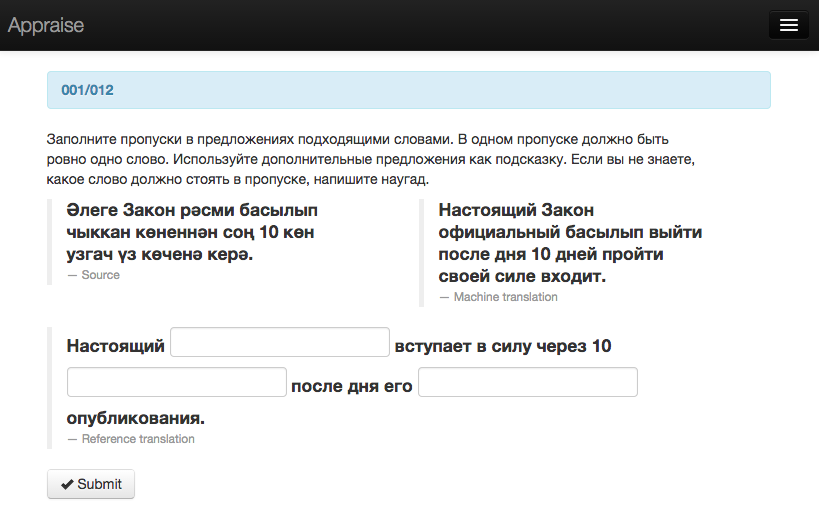
\includegraphics[width=1.0\textwidth,resolution=144]{appraise-scr}
 \caption{An example set of sentences in the online environment. The task is Russian legal text with 30\% gaps.}
\label{figure:screenshot}
\end{figure*}

In the course of the experiment, following \cite{oregan13}, we offer these hint combinations:
\begin{description}\itemsep 0ex
\item[Reference sentence only:] The participants are asked to fill the gaps without being given
any context. This task serves as a baseline score and as an indicator of gaps
that can be completed using common knowledge or language intuition (e.g.
idioms and strong collocations). For example, in an English phrase 'Jack ordered <...> and chips', one of the natural answers would be 'fish'. Such an answer, however, may be unrelated to the meaning of text, and may be given on the basis of collocation only.
\item[Reference sentence and source sentence:] By setup, the
participants have no command of the source language, however, it may help them to fill
in proper nouns or loan words.
\item[Reference sentence and MT hint:] In addition to the reference sentence, the
participants see the source sentence translated via the MT system, in this case Apertium \citep{forcada11}. This type of task is
used for measuring the contribution of machine translation to understanding the
gist of the text.
\item[Reference sentence and both hints:] This task is
added to check whether MT and source provide complementary hints.
\end{description}

In order to prepare the evaluation questions, we determine and remove keywords from the 
reference sentences. We consider two parameters: the list of allowed parts of speech (PoS), and the 
number of gaps relative to sentence length (``gap density''). For the evaluations described in 
this paper we use gap densities of 10, 20 and 30 percent (Table~\ref{table:percentage}), and the following parts of speech: noun (including proper nouns), adjective, adverb and lexical verb (as opposed to auxiliary verb).

For each sentence, the list of candidate keywords is prepared. It is composed of all the words that 
fall into the allowed PoS list. The number of gaps in the sentence is calculated based on 
sentence length and specified gap density. All reference sentences are longer than 10 words. Finally, the required number of keywords is selected 
from the candidate list in such a manner that the gaps are distributed evenly throughout the sentence. We start at a random word in a sentence and check whether it is a keyword candidate. If yes, we remove it, and move \emph{n} words forward, going back to the beginning of sentence if necessary. The step length \emph{n} is the sentence length divided by the desired number of gaps. If the word is not a keyword, or has already been removed, we look at the next word instead. The process is repeated until the designated number of words has been removed, or until there are no more words in the keyword list.
%\comment{MLF: O'Regan and Forcada did something lots simpler: why not here? It is probably a bit late to change this}

%\comment{MLF: the procedure described so far seems automatic. What's manual and time consuming?} 
Keyword removal could be one of the most time-consuming steps in task preparation. It normally requires human effort, because we would like to determine the words that contribute the most to understanding the text as opposed to removing random words. In our automatic setup, the above procedure is performed by a script integrated into the task generation pipeline. Parts of speech are determined with Apertium morphological analyser. To control for homonymy, we only allow the word into the candidate list if all of its possible part of speech attributions are on the PoS list. For example, if we only allow nouns on the word list, and the word "fly" receives two possible part of speech attributions from the tagger, noun and verb, it is not considered for the candidate list.

Having prepared the sentence sets, we assemble them into XML formatted for the Appraise platform.

\section{Experimental set-up}
\label{sec:setup}

In this section we will discuss the evaluators, the evaluation procedure, and the tasks in more detail.

For each experiment we called for native speakers of target language of the language pair (i.e.
Spanish and Russian) who had no command of source language of the pair (Basque
and Tatar, respectively). The knowledge was self-reported, and the participants were not asked about any other languages they may know. \comment{EA 12: should I elaborate on this? Write that Basque is not mutually understandable with anything? I am pretty sure we had no one from Tatarstan, but there may have been someone who knows some Bashkir, which might have helped them. Also, with Tatar, I think, Russian loanwords help more than anything else. } Eleven evaluators participated in the Basque--Spanish experiment, and 28 in Tatar-Russian (although not everyone completed the task
in full, see discussion). The majority of Russian participants were aged 20-25, with university degrees or in the process of obtaining them. Although we have not asked the participants about their knowledge of languages other than Tatar and Russian, it is reasonable to assume that most Russian participants knew English to some extent. \comment{EA 12: could you tell me more about the Spanish evaluators? I would write something similar}

By design, our gap-filling tasks require a human translation (reference) of source sentences. Calling for a human translator, however, would significantly increase the resources needed for evaluation. We therefore use parallel text sources, which provide the same sentence in two languages simultaneously:
\begin{enumerate}
\item  For Basque--Spanish, from the corpus of legal texts ``Memorias de traducci\'on del
Servicio Oficial de Traductores del IVAP'';\footnote{\url{http://tinyurl.com/ivaptm2}} 
\item  For Tatar-Russian, from the following sources on three different topics:
  \begin{enumerate}
    \item  Casual conversations, from a textbook\footnote{\rus{Литвинов И.Л. Я начинаю говорить по-татарски. Казань: Татарское кн. изд-во, 1994. — 320 с. ISBN 5--298--00463--6 (стр. 219, 220, 232, 233, 234)}} of spoken Tatar;
    \item  Legal texts, from the Constitution and laws\footnote{\url{http://tatarstan.ru}} of Tatarstan;
    \item  News, from the President of Tatarstan website\footnote{\url{http://president.tatarstan.ru/}}.
  \end{enumerate}
\end{enumerate}

Each set features 36 pairs of sentences. For the Basque--Spanish experiment the pairs were drawn
randomly from the corpora, for Tatar--Russian, compiled by hand by the developer of the
language pair in Apertium. The Basque--Spanish experiment featured 94, 181 and 272 gaps in the 10, 20 and 30 \% tasks, respectively. For Tatar--Russian these numbers are 272, 396 and 724, due to longer sentences used in task creation. \comment{EA to JA: Ilnar wanted to test the system on his own sentences, should I put it in the paper?}

\subsection{Procedure}

The evaluations took place online, in a system called Appraise \citep{federmann12}, which is 
designed specifically for various MT evaluation tasks. We adapted the code of Appraise to 
accommodate for the gap-filling tasks. The tasks were uploaded into the system and 
manually distributed between the participants by the following rules:
\begin{enumerate}
\item  Each participant evaluates every sentence (understood as a succession of words),
a total of 36;
\item  these sentences are divided into 4 groups of 9, one for each evaluation mode (see section~\ref{sec:methodology});
\item in total, all sentences of the set are evaluated with 10, 20 and 30\% of words removed;
\item each participant may encounter a given sentence in only one of the percentage variations;
\item  each sentence-mode-percentage combination is evaluated by more than one participant.
\end{enumerate}


The participants are given the instructions in their native language; these instructions are repeated above each task in the evaluation system. For the participants' convenience, the body of questions is split into smaller groups which allow multiple evaluation sessions. The instructions are the 
following: read all the available hints and fill each gap with one suitable word, guessing if unsure.
Participants' answers are recorded and marked correct or incorrect automatically. \comment{EA 11,16: should I try to clarify this? one of the reviewers thought it was manual work}In
addition, the time taken to fill the gaps in one sentence is recorded.

This variety of the gap-filling task requires open answers, and it is therefore possible that the participants may
provide words that fit the gaps well, but do not match the original answer. To account for
these cases, we process all the answers to detect possible synonyms (a method suggested by \cite{oregan13}). An answer is
considered a candidate synonym if it is given by two or more evaluators, and it does not match
the answer word. We record each candidate synonym along with the answer key and the
context sentence. For example, the word \emph{asumir} is the original answer in the Spanish sentence \emph{Aprender a jugar y divertirse en el agua sin asumir riesgos} ('Learning to play and have fun in the water without taking risks'). However, two or more evaluators gave a different answer, \emph{correr} (\emph{correr riesgos}, 'running risks'). Based on this data, an expert, who is native speaker of the target language and who has not participated in the evaluations, decides
whether the candidate synonym is an acceptable replacement to the answer key in the given
context. We then check participants' results against the compiled synonym list and
increase scores where appropriate. On average, the scores improved by three percentage points in all evaluation modes. Candidate synonyms are extracted automatically from the evaluators' responses,  and each individual score is automatically updated according to the synonym list.

The synonym lists for Basque--Spanish and Tatar--Russian contain 52 and 25 words, respectively. The time taken to compile each list depends on the number of candidate synonyms, and in our case was approximately 30 minutes. 

\section{Results and discussion}
\label{sec:results}
\begin{table*}
\centering
  \begin{tabular}{|l|r|r|r|r|r|r|r|r|}
  \hline
 \multirow{2}{*}{\textbf{Density}} & \multicolumn{4}{|c|}{Basque--Spanish} & \multicolumn{4}{|c|}{Tatar--Russian} 
\\\cline{2-9}
                                            & \textbf{MT \& Src} & \textbf{MT} & \textbf{Src} & \textbf{No hint}& \textbf{MT \& Src} & \textbf{MT} & \textbf{Src} & \textbf{No hint} 
\\
\hline
10\%&62 \(\pm\) 32&58 \(\pm\) 28&40 \(\pm\) 39&49 \(\pm\) 40
&57 \(\pm\) 42&64 \(\pm\) 41&54 \(\pm\) 43&46 \(\pm\) 41\\
20\%&65 \(\pm\) 30&70 \(\pm\) 27&31 \(\pm\) 28&31 \(\pm\) 30
&65 \(\pm\) 31&60 \(\pm\) 33&46 \(\pm\) 31&39 \(\pm\) 32\\
30\%&48 \(\pm\) 26&40 \(\pm\) 24&26 \(\pm\) 20&18 \(\pm\) 18
&59 \(\pm\) 28&56 \(\pm\) 26&40 \(\pm\) 28&35 \(\pm\) 30\\
\hline
\end{tabular}
\caption{Average number of gaps successfully filled (\%), using a synonym list} 
\label{table:res}
\end{table*}

The results are presented in this section. Table \ref{table:res} 
shows
the proportion and standard deviation of correct answers depending on evaluation mode and gap density.
The evaluators' correct answer percentage is averaged over the number of evaluators. In addition to the percentage of correct answers we kept a record of the time taken to fill the gaps in one sentence. To reduce the noise from participants who were distracted during evaluation, when
calculating times we remove all the results over 6 minutes (the statistical mode is approximately
two minutes). The typical time taken to complete one question varies from under one minute for tasks without hints and few gaps, to approximately two minutes for tasks with more hints and gaps. 

% expected results
We expect to see the following trend: scores received in different task modes inside one gap density should be observed, from highest to lowest, in tasks with MT and source hint, then MT hint only, then source hint only, and finally, no hint. We also expect that with the increase in gap density, the time taken to fill the gaps should also increase, and the percentage of correct answers should decrease. 

% a few notes on time
The latter trend holds: the average time taken to fill the gaps increases and the average percentage of correct answers decreases as the relative number of gaps goes up. The larger number of gaps in the sentence makes it more
difficult to predict the answer based on the context, and also leaves more room for
mistakes. Exploring different percentage-mode combinations, we may note that the 10\% no-hint tasks take the least time to complete. We would have expected longer completion time, since the participant must come up with their own answer unassisted. However, in the no-hint task the participant is required to read only one (reference) sentence, as opposed to two or three (reference and hints) in other tasks. Also, the number of gaps in 10\%-gap tasks is low, as it never exceeds three. We found that, as opposed to trying to devise the best word for no-hint gaps, the participants often resorted to filing these gaps with random words, which takes little time.

% this section talks about percentages in eu-es and tat-rus, and how everything is nice.
We will now discuss the percentage of correct answers based on task type. In general, tasks with MT hints score higher than tasks without MT hints. This aligns well with our expectations and suggests than machine translation helps to understand the provided text. In addition, tasks with source hints are completed better than tasks without hints, and the same relation holds between MT+source and MT-only types of tasks. In view of the relatively large standard deviations, the significance of the hints' contribution was tested using a linear regression model. The data points were represented as an individual evaluator's average score (the number of correct answers divided by the total number of answers) in each of the percentage-hint combinations. Two separate models were created: one for no-hint vs MT-hint tasks, and another for no-hint vs source-hint tasks. Given the null hypothesis of the regression line slope equal to zero, the contribution of MT hint is significant on the p~<~0.001 level. The contribution of the source hint is insignificant with p~=~0.162.

Two records in the data do not align with our expectations: the no-hint 10\% sentences in Basque--Spanish, which scored significantly higher than the source-hint in the same category, and MT+source 10\% sentences in Tatar--Russian, which we would have expected to score higher than the corresponding MT task. In the first case, this is largely due to the use of synonyms list. Before taking synonyms into account, the scores were 32 and 35 percent for source and no-hint tasks, respectively. This still shows a small difference in favor of no-hint tasks. However, the latter percentage increases significantly after we extend the answer list with synonyms. Such an increase suggests that, in this case, the content words were restored by 
semantic context rather than through strong collocation. The second pattern, low scores in Tatar--Russian 10\% MT+source, does not stem from the task content. Instead, it is the result of the fixed order of tasks: the participants have always been given MT+source 10\% sentences first, followed by other task types.\comment{MLF: Why? Not random? \cite{oregan13} did random! Why was this changed?}The participants have not received any training tasks before the main evaluations. Therefore, it is possible that the accommodation period is responsible for lower-than-expected scores in this mode of evaluation. 

It remains questionable whether we can compare results for different gap densities. The 10, 20 and 30\% sets were comprised
of the same sentences. However, in each case different words were removed. It appears
that some content words are easier to fill than the others. This may explain why in
Basque--Spanish the 20\% MT tasks are completed with better accuracy than 10\% tasks.\comment{MLF: I think this shows that our statistics are weak, should we say something to excuse ourselves?}

It is worth noting that many participants reported feeling frustrated in
the course of evaluations, especially while working on the no-hint tasks. The latter required suggesting the words with very little context, which led some of the participants to giving random words for answers, or leaving the space blank. 6 out of 49
participants quit the experiment before completing it. Considering the importance of receiving the full set of evaluations, we must address the issue of participant motivation in the upcoming experiments. It may be beneficial to offer monetary compensation for the evaluators' efforts (in our case, they were volunteers).

\subsection{Annotator agreement}
After obtaining the results we calculated Krippendorff's alpha~\citep{krippendorff70} measure to represent annotator agreement, shown in Table~\ref{table:alpha}. 
\begin{table*}
\centering
  \begin{tabular}{|l|r|r|r|r|r|r|r|r|}
  \hline
 \multirow{2}{*}{\textbf{Density}} & \multicolumn{4}{|c|}{Basque--Spanish}&\multicolumn{4}{|c|}{Tatar--Russian} \\\cline{2-9}
                                            & \textbf{MT \& Src} & \textbf{MT} & \textbf{Src} & \textbf{No hint}& \textbf{MT \& Src} & \textbf{MT} & \textbf{Src} & \textbf{No hint} \\
\hline
10\%&0.496&0.517&0.400&0.124&0.598&0.459 &0.711 &0.517\\
20\%&0.714&0.700&0.358&0.275&0.740&0.667 &0.473 &0.261\\
30\%&0.559&0.430&0.406&0.300&0.534&0.581 &0.411 &0.412\\

\hline
\end{tabular}
\caption{Krippendorff Alpha measure} 
\label{table:alpha}
\end{table*}

We selected this measure because of its compatibility with more than two annotators per task and the missing data (not all the gaps were evaluated). To calculate Krippendorff's alpha we used an algorithm implementation by Thomas Grill,\footnote{\url{http://grrrr.org/data/dev/krippendorff_alpha/}} dividing the answers in each gap into two categories: correct and incorrect. The previously obtained synonym lists were taken into account, i.e. if the two answers are different but both correct, they fall into one category. The measure was calculated separately for each hint and percentage combination.

The interpretation of Krippendorff's alpha varies depending on the application. One of the general guidelines suggested by \citet{landis77} for kappa-like measures (which includes Krippendorff's Alpha) is as follows: k < 0.00 indicates ``poor'' agreement, 0.00 to 0.20 ``slight'', 0.21 to 0.40 ``fair'', 0.41 to 0.60 ``moderate'', 0.61 to 0.80 ``substantial'', and 0.81 to 1.00 ``near perfect''.

In general, the level of annotator agreement is relatively high. As the MT and MT+source hints are introduced, the agreement increases (measures closer to 1): the annotators are more consistently correct or incorrect in each given sentence. The agreement measure for the same sentences without hints is closer to zero, which contributes to the reliability of our methodology. We note the outlier score in Tatar--Russian 10\% source tasks, which has the most contribution from the news texts. \comment{EA: this Alpha is from a table we do not report here, I added a couple of words to clarify}This set of sentences contains many loan words, which have similar form in Tatar and Russian (e.g. president, minister, championship), and are understood by Russian speakers. The gaps with loan words have mostly been filled correctly, while there was some disagreement in other gaps.

% a little on categories
\subsection{Results for different domains}
\begin{table*}
\centering
\begin{tabular}{|r|r |*{4}{c}|}
\hline
\multicolumn{2}{|c|}{} &\multicolumn{4}{c|}{\textbf{Evaluation mode}}\\
\hline
\textbf{Domain} & \textbf{Gap percentage} & \textbf{MT \& Src} & \textbf{MT} & \textbf{Src} & \textbf{No hint} \\
\hline
 \multirow{3}{*}{\textbf{Casual}} &
10\%&64 \(\pm\) 45&64 \(\pm\) 43&62 \(\pm\) 46&53 \(\pm\) 44\\
& 20\%&73 \(\pm\) 32&63 \(\pm\) 36&41 \(\pm\) 28&38 \(\pm\) 31\\
& 30\%&70 \(\pm\) 31&60 \(\pm\) 24&39 \(\pm\) 27&38 \(\pm\) 33\\
\hline
 \multirow{3}{*}{\textbf{Legal}} &
10\%&53 \(\pm\) 40&68 \(\pm\) 35&39 \(\pm\) 38&33 \(\pm\) 35\\
&20\%&61 \(\pm\) 25&66 \(\pm\) 24&50 \(\pm\) 34&48 \(\pm\) 34\\
&30\%&50 \(\pm\) 26&48 \(\pm\) 29&40 \(\pm\) 27&34 \(\pm\) 29\\
\hline
 \multirow{3}{*}{\textbf{News}} &
10\%&53 \(\pm\) 38&60 \(\pm\) 44&57 \(\pm\) 42&49 \(\pm\) 39\\
&20\%&59 \(\pm\) 34&49 \(\pm\) 35&47 \(\pm\) 32&29 \(\pm\) 29\\
&30\%&58 \(\pm\) 22&61 \(\pm\) 22&41 \(\pm\) 30&35 \(\pm\) 27\\
\hline

\end{tabular}
\caption{Tatar--Russian Average number of gaps successfully filled (\%), using a synonym list, for three different domains.} 
\label{table:rus} 
\end{table*}

For the Tatar--Russian language pair the participants were offered texts from three different domains (in equal proportions): casual conversations, legal texts and news. The results by domains are displayed in table~\ref{table:rus}. The MT system used in the evaluation has been targeted to translate texts from all three of the domains. Taking into consideration the above discussion of 10\% MT+Source tasks, we observe similar results across the three categories. Note that the source sentences paired with MT improve participants' performance in casual texts, compared to MT-only task mode. This may be due to the fact that many words are borrowed from Russian into Tatar, and are in fact understood by Russian speakers.

% results with synonyms

% \begin{table*}
% \centering
%   \begin{tabular}{|l|r|r|r|r|}
%   \hline
%  \multirow{2}{*}{\textbf{Density}} & \multicolumn{4}{|c|}{Evaluation mode} \\\cline{2-5}
%                                             & \textbf{MT \& Src} & \textbf{MT} & \textbf{Src} & \textbf{No hint} \\
% \hline
% 10\%&62 \(\pm\) 32&58 \(\pm\) 28&40 \(\pm\) 39&49 \(\pm\) 40\\
% 20\%&65 \(\pm\) 30&70 \(\pm\) 27&31 \(\pm\) 28&31 \(\pm\) 30\\
% 30\%&48 \(\pm\) 26&40 \(\pm\) 24&26 \(\pm\) 20&18 \(\pm\) 18\\
% \hline
% \end{tabular}
% \caption{Basque--Spanish: Average number of gaps successfully filled (\%), using a synonym list} 
% \label{table:res-eus-spa}
% \end{table*}


% \begin{table*}
% \centering
%   \begin{tabular}{|l|r|r|r|r|}
%     \hline
%     \multirow{2}{*}{\textbf{Density}} & \multicolumn{4}{|c|}{Evaluation mode} \\\cline{2-5}
%                                             & \textbf{MT \& Src} & \textbf{MT} & \textbf{Src} & \textbf{No hint} \\
% \hline
% 10\%&57 \(\pm\) 42&64 \(\pm\) 41&54 \(\pm\) 43&46 \(\pm\) 41\\
% 20\%&65 \(\pm\) 31&60 \(\pm\) 33&46 \(\pm\) 31&39 \(\pm\) 32\\
% 30\%&59 \(\pm\) 28&56 \(\pm\) 26&40 \(\pm\) 28&35 \(\pm\) 30\\
%     \hline
%   \end{tabular}
%   \caption{Tatar--Russian: Average number of gaps successfully filled (\%), using a synonym list}
%   \label{table:res-tat-rus}
% \end{table*}

% \begin{table*}
% \centering
%   \begin{tabular}{|l|r|r|r|r|}
%   \hline
%  \multirow{2}{*}{\textbf{Density}} & \multicolumn{4}{|c|}{Evaluation mode} \\\cline{2-5}
%                                             & \textbf{MT \& Src} & \textbf{MT} & \textbf{Src} & \textbf{No hint} \\
% \hline
% 10\%&0.496&0.517&0.400&0.124\\
% 20\%&0.714&0.700&0.358&0.275\\
% 30\%&0.559&0.430&0.406&0.300\\

% \hline
% \end{tabular}
% \caption {Basque--Spanish: Krippendorff Alpha measure} 
% \label{table:alpha-eus-spa}
% \end{table*}



% \begin{table*}
% \centering
%   \begin{tabular}{|l|r|r|r|r|}
%   \hline
%  \multirow{2}{*}{\textbf{Density}} & \multicolumn{4}{|c|}{Evaluation mode} \\\cline{2-5}
%                                             & \textbf{MT \& Src} & \textbf{MT} & \textbf{Src} & \textbf{No hint} \\
% \hline
% 10\%&0.598&0.459 &0.711 &0.517 \\
% 20\%&0.740&0.667 &0.473 &0.261 \\
% 30\%&0.534&0.581 &0.411 &0.412 \\
% \hline
% \end{tabular}
% \caption {Tatar--Russian: Krippendorff Alpha measure} 
% \label{table:alpha-tat-rus}
% \end{table*}

% results by text mode in tat-rus, with synonyms
% \begin{table*}
% \centering
% \begin{tabular}{|r|r |*{4}{c}|}
% \hline
%   &&\multicolumn{4}{c|}{\textbf{Evaluation mode}}\\
% \hline
% & \textbf{Gap percentage} & \textbf{MT \& Src} & \textbf{MT} & \textbf{Src} & \textbf{No hint} \\
% \hline
%  \multirow{3}{*}{\textbf{Casual}} &
% 10\%&64 \(\pm\) 45&64 \(\pm\) 43&62 \(\pm\) 46&53 \(\pm\) 44\\
% & 20\%&73 \(\pm\) 32&63 \(\pm\) 36&41 \(\pm\) 28&38 \(\pm\) 31\\
% & 30\%&70 \(\pm\) 31&60 \(\pm\) 24&39 \(\pm\) 27&38 \(\pm\) 33\\
% \hline
%  \multirow{3}{*}{\textbf{Legal}} &
% 10\%&53 \(\pm\) 40&68 \(\pm\) 35&39 \(\pm\) 38&33 \(\pm\) 35\\
% &20\%&61 \(\pm\) 25&66 \(\pm\) 24&50 \(\pm\) 34&48 \(\pm\) 34\\
% &30\%&50 \(\pm\) 26&48 \(\pm\) 29&40 \(\pm\) 27&34 \(\pm\) 29\\
% \hline
%  \multirow{3}{*}{\textbf{News}} &
% 10\%&53 \(\pm\) 38&60 \(\pm\) 44&57 \(\pm\) 42&49 \(\pm\) 39\\
% &20\%&59 \(\pm\) 34&49 \(\pm\) 35&47 \(\pm\) 32&29 \(\pm\) 29\\
% &30\%&58 \(\pm\) 22&61 \(\pm\) 22&41 \(\pm\) 30&35 \(\pm\) 27\\
% \hline

% \end{tabular}
% \caption{Tatar--Russian Average number of gaps successfully filled (\%), using a synonym list, for three different domains.} 
% \label{table:rus} 
% \end{table*}



% \begin{table*}

% \centering
% \begin{tabular}{|r |*{4}{c}|}
% \hline
%   &\multicolumn{4}{c|}{\textbf{Evaluation mode}}\\
% \hline
% \textbf{Gap percentage} & \textbf{MT \& Src} & \textbf{MT} & \textbf{Src} & \textbf{No hint} \\
% \hline
% 10\%&64 \(\pm\) 45&64 \(\pm\) 43&62 \(\pm\) 46&53 \(\pm\) 44\\
% 20\%&73 \(\pm\) 32&63 \(\pm\) 36&41 \(\pm\) 28&38 \(\pm\) 31\\
% 30\%&70 \(\pm\) 31&60 \(\pm\) 24&39 \(\pm\) 27&38 \(\pm\) 33\\
% \hline
% \end{tabular}
% \caption {Tatar--Russian, casual conversations: Average number of gaps successfully filled (\%), using a synonym list} 
% \label{table:rus-casual} 
% \end{table*}

% \begin{table*}
% \centering
% \begin{tabular}{|r |*{4}{c}|}
% \hline
%   &\multicolumn{4}{c|}{\textbf{Evaluation mode}}\\
% \hline
% \textbf{Gap percentage} & \textbf{MT \& Src} & \textbf{MT} & \textbf{Src} & \textbf{No hint} \\
% \hline
% 10\%&53 \(\pm\) 40&68 \(\pm\) 35&39 \(\pm\) 38&33 \(\pm\) 35\\
% 20\%&61 \(\pm\) 25&66 \(\pm\) 24&50 \(\pm\) 34&48 \(\pm\) 34\\
% 30\%&50 \(\pm\) 26&48 \(\pm\) 29&40 \(\pm\) 27&34 \(\pm\) 29\\
% \hline
% \end{tabular}
% \caption {Tatar--Russian, legal texts: Average number of gaps successfully filled (\%), using a synonym list} \label{table:rus-legal} 
% \end{table*}

% \begin{table*}
% \centering
% \begin{tabular}{|r |*{4}{c}|}
% \hline
%   &\multicolumn{4}{c|}{\textbf{Evaluation mode}}\\
% \hline
% \textbf{Gap percentage} & \textbf{MT \& Src} & \textbf{MT} & \textbf{Src} & \textbf{No hint} \\
% \hline
% 10\%&53 \(\pm\) 38&60 \(\pm\) 44&57 \(\pm\) 42&49 \(\pm\) 39\\
% 20\%&59 \(\pm\) 34&49 \(\pm\) 35&47 \(\pm\) 32&29 \(\pm\) 29\\
% 30\%&58 \(\pm\) 22&61 \(\pm\) 22&41 \(\pm\) 30&35 \(\pm\) 27\\
% \hline
% \end{tabular}
% \caption {Tatar--Russian, news: Average number of gaps successfully filled (\%), using a synonym list} 
% \label{table:rus-news} 
% \end{table*}

\section{Conclusions}
\label{sec:conclusion}
We have conducted assimilation evaluation of two Apertium translation directions: Basque--Spanish and Tatar--Russian. The results suggest that this evaluation method reflects the contribution of MT to users' understanding of text. The version of the toolkit used in this 
experiment may be downloaded from our repository.\footnote{{\url{https://github.com/Sereni/Appraise/tree/1e9d735faee64d1b97fb343ab111ace6a64509d7}}}

The experiments may easily be repeated for any language pair (provided a parallel corpus) and
any machine translation system. Based on our experience, we would like to suggest the following amendments to the procedure:
\begin{enumerate}
\item As reported in \cite{oregan13}, unless the evaluation is targeted at a specific text domain, it may be beneficial to include a stylistic variety of texts in the initial corpus. Neighboring sentences on the same topic may assist the users in gap-filling tasks;
\item If possible, increase the number of evaluators, or reduce the number of questions per participant. In the above experiments each participant filled from 110 to 187 gaps, divided into small groups. Reducing the amount of work may increase task completion rate;\comment{MLF's crazy idea: recaptchas?}\comment{EA: the participants did not leave the gaps empty, they just did not attempt the next portions of evaluation after finishing some and getting bored. or did I misunderstand the use of captchas? }
\item To account for the adaptation period, provide training tasks before the main evaluations take place.
\end{enumerate}

As a consideration for future work, it may be beneficial to compare the results of evaluation by gap-filling method with the traditional evaluation metrics, as well as with human evaluation.

\section*{Acknowledgments}

This work has been partly funded by the Spanish Ministerio de Econom{\'i}a y Competitividad through project TIN2012-32615 and by the Google Summer of Code 2014 programme. Ekaterina Ageeva's work has been supported by Google Summer of Code 2014 through the Apertium project. We would like to thank the volunteers who participated in the evaluations.

\bibliographystyle{apalike}

\comment{EA: urls do not show up in web citations, how can I fix that?}
\bibliography{2015-eamt-assim}

\end{document}
